\chapter{運動量保存則}

前章で学んだ「力学的エネルギー保存則」は, うまく使えば, 運動方程式を
解かなくても, 物体の運動について多くのことを簡単に教えてくれる。しかし, 
あの法則にも弱点がある。ひとつは, 摩擦力などの非保存力が働いてたら
使えない, ということ。もうひとつは, 物体の「速さ」は教えてくれても
「運動の方向」は教えてくれないことである。

そこで, それらを補ってくれるような, もうひとつの保存則をここでは学ぶ。
それは「運動量保存則」である。この法則もいくつか弱点があるが, 
力学的エネルギー保存則が使えない時にも使える(ことがある)し、
力学的エネルギー保存則と組み合わせることができれば, さらに威力を
発揮する。\\

特に強力なのは, 複数の物体どうしが衝突するような状況である。\\

\section{運動量保存則}\index{うんどうりょうほぞんそく@運動量保存則}

図\ref{fig:collision}のような, 2つの質点A, Bが近づいてきて
衝突し, 一体化する運動を考える。質点A, Bそれぞれの質量を$m_{\text A}, m_{\text B}$
とする。時刻$t_0$のとき(衝突前), 質点A, Bはそれぞれ速度${\bf v}_{\text A}, {\bf v}_{\text B}$
で$xy$平面上を別の方向に等速直線運動しているとしよう。
時刻$t_1$に2つは衝突して合体する。そして時刻$t_2$では(衝突後), 
合体した物体が新たな方向に速度${\bf v}$で進んでいるとしよう。
この速度${\bf v}$を求めよ, と言われたらどうすればよいだろう?

\begin{figure}[h]
    \centering
    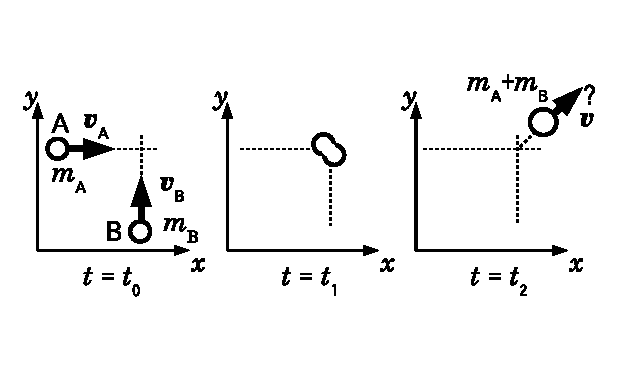
\includegraphics[width=7.0cm]{collision.eps}
    \caption{2つの質点の衝突合体}\label{fig:collision}
\end{figure}

極微の世界や高速の世界を除けば, どんな運動も運動方程式に従うので, 
この件も運動方程式を解けば完璧に予測・解明できるはずだ。
しかし, この件に関しては, 運動方程式を正面から解くのは難しい。
というのも, そもそも「衝突して合体」は, 時刻$t_1$の「瞬間」で起きるのではなく, 
衝突が始まって物体が徐々につぶれて, その間, 弾性力や摩擦力が
複雑に働き, やがてお互いがくっつきあって一体化するまで, 短い時間
だが複雑な現象が起きるのだ。その各時刻に, 2つの物体の間に
どのように力が働くのかを解明するのは大変難しい作業だ。

というわけで, この時刻$t_1$付近で起きる「衝突して合体」という複雑な
現象を運動方程式で直接扱うことは避けたい。君子危うきに近寄らず, 
と言うではないか。\mv

そこで有用なのが, これから学ぶ, 以下の法則である:
\begin{itembox}{運動量保存則}
外力が働かない系では, 全運動量(各質点の運動量の総和)は不変である。
\end{itembox}
外力とは, 考察の対象になっている物体どうしに働く力(それを内力という)
以外の力だ。本件でも外力は働いていない
\footnote{衝突して合体するまでに生じる複雑な力は, 
具体的にその力がどんなものなのかというのは置いといて, 
「考察の対象になっている物体どうしに働く力」なので内力である。}。
全運動量とは, 各物体の運動量の(ベクトルとしての)和である。
運動量とは, \eref{eq:def_momentum}で定義されたように, 質量と速度の積である。

この法則がなぜ成り立つかは, 後で説明するとして, とりあえずこの法則が正しいと
信じてみよう。本件では, 時刻$t_0$(つまり衝突前)の全運動量は, 
\begin{eqnarray} 
m_{\text A}{\bf v}_{\text A}+m_{\text B}{\bf v}_{\text B}\label{eq:momentum_mAmB_0}
\end{eqnarray} 
である。ここで, 添字のA, Bは, それぞれ質点A, 質点Bの属性であることを示す。
時刻$t_2$(つまり衝突後)では質点はひとつに合体しており, その運動量は, 
\begin{eqnarray} 
(m_{\text A}+m_{\text B}){\bf v}\label{eq:momentum_mAmB_1}
\end{eqnarray} 
である。運動量保存則は, \eref{eq:momentum_mAmB_0}と\eref{eq:momentum_mAmB_1}
が等しい, と主張するのだ。すなわち, 
\begin{eqnarray} 
m_{\text A}{\bf v}_{\text A}+m_{\text B}{\bf v}_{\text B}=(m_{\text A}+m_{\text B}){\bf v}
\end{eqnarray} 
が成り立つはずだ。それを認めるなら, 
\begin{eqnarray} 
{\bf v}=\frac{m_{\text A}{\bf v}_{\text A}+m_{\text B}{\bf v}_{\text B}}{m_{\text A}+m_{\text B}}\label{eq:2body_adhere}
\end{eqnarray} 
となって, 衝突後の質点の速度が求まる。実際, 実験してみると, 確かにこうなるのだ。\mv

%
\begin{q}\label{q:collision0}
図\ref{fig:collision}の問題において, $m_{\text A}=m_{\text B}=1.0$~kgとし, 時刻$t_0$でAは$x$軸
方向に1.0~m s$^{-1}$, Bは$y$軸方向に1.0~m s$^{-1}$で動いているとする。
\begin{enumerate}
\item 衝突合体後の速度${\bf v}$を求めよ。
\item $|{\bf v}|$を求めよ。
\end{enumerate}
\end{q}\mv

では, 運動量保存則を証明しよう。まず運動方程式に戻る(運動の話は全て運動方程式から始まるのだ!)。
質量$m$の質点が力${\bf F}$を受けて
運動しているとき, その運動は, どんなものでも以下の運動方程式に従う:
\begin{eqnarray}{\bf F}=m{\bf a}=m\frac{d{\bf v}}{dt}=m\frac{d^2{\bf r}}{dt^2}\end{eqnarray}
$t$は時刻である。${\bf r}, {\bf v}, {\bf a}$は
それぞれ, 質点の位置, 速度, 加速度。さて, 上の式は, 以下のように書ける:
\begin{eqnarray} 
m\frac{d{\bf v}}{dt}={\bf F}\label{eq:maF}
\end{eqnarray} 
両辺に$dt$をかけると次式になる:
\begin{eqnarray} 
m\,d{\bf v}={\bf F}\,dt\label{eq:consmom_mdv_Fdt}
\end{eqnarray} 
これを時刻$t=t_0$から時刻$t=t_1$まで$t$で積分すれば, 
\begin{eqnarray} 
\int_{{\bf v}(t_0)}^{{\bf v}(t_1)}m\,d{\bf v}=\int_{t_0}^{t_1}{\bf F}\,dt\label{eq:momentum_00}
\end{eqnarray} 
となる。左辺は, 
\begin{eqnarray} 
\Bigl[m{\bf v}\Bigr]_{{\bf v}(t_0)}^{{\bf v}(t_1)}=m{\bf v}(t_1)-m{\bf v}(t_0)
\end{eqnarray} 
となるから, \eref{eq:momentum_00}は, 
\begin{eqnarray} 
m{\bf v}(t_1)-m{\bf v}(t_0)=\int_{t_0}^{t_1}{\bf F}\,dt\label{eq:momentum1}
\end{eqnarray} 
となる。この式の左辺は「時刻$t_0$から$t_1$の間に運動量がどれだけ変わったか」だ。
一方, 右辺は\underline{力積}\index{りきせき@力積}(りきせき, と読む)と
いう量である。
\begin{itembox}{力積の定義}
時刻を$t$とする。質点に, 力${\bf F}(t)$が働くとき, 
\begin{eqnarray}
\int_{t_0}^{t_1}{\bf F}\,dt\label{eq:rikiseki}
\end{eqnarray}
を, 時刻$t_0$から$t_1$までに質点に働く力積と呼ぶ。
\end{itembox}

\begin{q}\label{q:def_rikiseki}
力積の定義を5回書いて記憶せよ。\end{q}\mv

すなわち, \eref{eq:momentum1}は, 「\textgt{運動量の変化は力積に等しい}」と解釈できる。これはこれで大切な法則である。そして, この法則をもとに, 運動量保存則が証明される(ちなみに, この法則のことを運動量保存則と呼ぶこともある)。

\begin{faq}{\small\textgt{「運動エネルギーの変化は仕事に等しい」という法則と似てますね}
... 似てるけど違います。両者の違いをきちんと認識しよう。運動エネルギーや仕事はスカラーで, その法則は運動方程式
を位置で積分して得られました。一方, 運動量や力積は\textgt{ベクトル}で, ここで述べた法則は
運動方程式を\textgt{時刻で}積分することで得られたのです。}\end{faq}\mv

さて, いま, A, Bという2つの質点が互いに力を及ぼしあいながら時刻$t=t_0$から時刻$t=t_1$まで
運動する状況を考えよう。
各質点は外力を受けることがないとする。
質点Aが質点Bから受ける力を${\bf F}_{\text {AB}}$, とし, 
質点Bが質点Aから受ける力を${\bf F}_{\text {BA}}$とする。それぞれの質点に関して, \eref{eq:momentum1}
と同様の式が成り立つはずである:
\begin{eqnarray}
&&m_{\text A}{\bf v}_{\text A}(t_1)-m_{\text A}{\bf v}_{\text A}(t_0)=\int_{t_0}^{t_1}{\bf F}_{\text {AB}}dt\label{eq:momentumA}\\
&&m_{\text B}{\bf v}_{\text B}(t_1)-m_{\text B}{\bf v}_{\text B}(t_0)=\int_{t_0}^{t_1}{\bf F}_{\text {BA}}dt\label{eq:momentumB}
\end{eqnarray}
これらを辺々足し合わせると, 
\begin{eqnarray}
&&m_{\text A}{\bf v}_{\text A}(t_1)-m_{\text A}{\bf v}_{\text A}(t_0)+m_{\text B}{\bf v}_{\text B}(t_1)-m_{\text B}{\bf v}_{\text B}(t_0)\nonumber\\
&&=\int_{t_0}^{t_1}{\bf F}_{\text {AB}}dt+\int_{t_0}^{t_1}{\bf F}_{\text {BA}}dt\nonumber\\
&&=\int_{t_0}^{t_1}({\bf F}_{\text {AB}}+{\bf F}_{\text {BA}})\,dt\label{eq:momentumABsum}
\end{eqnarray}
となる。ここで作用反作用の法則から, 
\begin{eqnarray} 
{\bf F}_{\text {AB}}=-{\bf F}_{\text {BA}}
\end{eqnarray} 
である。従って, 
\begin{eqnarray} 
{\bf F}_{\text {AB}}+{\bf F}_{\text {BA}}={\bf 0}
\end{eqnarray}
である。従って, \eref{eq:momentumABsum}の最後の行は${\bf 0}$になる(${\bf 0}$の積分は${\bf 0}$)。従って, 
\begin{eqnarray*} 
m_{\text A}{\bf v}_{\text A}(t_1)-m_{\text A}{\bf v}_{\text A}(t_0)+m_{\text B}{\bf v}_{\text B}(t_1)-m_{\text B}{\bf v}_{\text B}(t_0)={\bf 0}
\end{eqnarray*}
となる。書き換えれば, 
\begin{eqnarray} 
m_{\text A}{\bf v}_{\text A}(t_1)+m_{\text B}{\bf v}_{\text B}(t_1)\nonumber\\
=m_{\text A}{\bf v}_{\text A}(t_0)+m_{\text B}{\bf v}_{\text B}(t_0)\label{eq:consmom000}
\end{eqnarray} 
となる。この式は, 2つの質点の運動量の和は時刻$t_1$と時刻$t_0$で変わらない, ということだ。
以上から, 「2つの質点が, 外力の影響を受けずに運動する場合, 全運動量は不変である」ということ
が示された。次の問で証明するように, 質点が3つになっても, 同様の式が成り立つ。この証明を, 
任意の個数の質点に拡張することも容易にできる。つまり, 前述の運動量保存則が成り立つ!

%
\begin{q}\label{q:3body_momentum}
3つの質点A, B, Cが互いに内力のみを受けて運動する系でも, 全運動量が保存する
ことを示せ。ヒント:式(\ref{eq:momentumA})のような式を, A, B, Cのそれぞれに
ついて考え, 足し合わせればよい。ただし, Aに働く力は${\bf F}_{\text {AB}}+{\bf F}_{\text {AC}}$
であることに注意。
\end{q}

\begin{q} 2つの質点A, Bが, $x$軸上を互いに逆向きに等速直線運動で運動し, 接近し, 
いずれ衝突する。質点A, Bの質量はそれぞれ2.0~kgと3.0~kgであり, 
衝突前の質点A, Bの速度はそれぞれ$-4.0$~m~s$^{-1}$, $5.0$~m~s$^{-1}$である。
衝突後, 2つの質点はくっついて1つの質点になる場合, 衝突後のこの質点の速度を求めよ。\end{q}
\hv


\section{衝突のときエネルギーはどうなるのか?}

この「運動量保存則」は, 前章までに学んだ「力学的エネルギー保存則」になんとなく似ているが, 
正直なところ, どう違うのだろうか? そこで, 以下の問を考えよう:

%
\begin{q}\label{q:collision1}
問\ref{q:collision0}の続きを考える。
\begin{enumerate}
\item 衝突前の運動エネルギーの総和を求めよ。
\item 衝突合体後の運動エネルギーを求めよ。
\end{enumerate}
\end{q}

この現象では, 衝突合体で運動エネルギーが減ってしまった。では, この減ったぶん
のエネルギーはどこに行ってしまったのだろう?

まず考えられるのは, ポテンシャルエネルギーである。既に学んだ「力学的エネルギー
保存則」では, 運動エネルギーとポテンシャルエネルギーの総和は一定なのだから, 
運動エネルギーが減った分, ポテンシャルエネルギーが増えていれば, つじつまは合う。

しかし! この衝突ではポテンシャルエネルギーは変化していない。ていうか, 外力が
無いからそもそもポテンシャルエネルギーは0である。もし外力(ボールの衝突における重力など)
があったらどうだろう? 外力が仕事をすれば, それはポテンシャル
エネルギーを変化させるだろう。ところが, 衝突の短い瞬間だけに注目すると, 
物体の運動は小さい空間領域で発生するので, たとえ外力があっても, 外力に
よる仕事はほとんど無視できる(仕事=力$\times$変位の「変位」が小さいから!)。
従って, 外力がある場合でも, 衝突の前後で外力によるポテンシャルエネルギー
の変化はほぼ0だ。従って, 外力があろうがなかろうが, 衝突の前後でポテンシャル
エネルギーは変化しない。

ならば外力以外の力によるポテンシャルエネルギーはどうだろう? 例えば, ボールどうし
が衝突するとき, ボールは変形する。その変形は, ボールを構成する各部分の弾性力
に逆らって行われる(仕事がされる)ものなので, 弾性力によるポテンシャルエネルギーを
増加させる。しかもこの変形は, 衝突終了後も, ボールをぐにゃぐにゃと振動させる
ことによって継続する。弾性力によるポテンシャルエネルギーは, この振動の運動エネルギー
にも転化するだろう。

そのような振動は, やがて収まるだろう。それは, ボール内部の摩擦によるものである。
そのとき, 振動のエネルギーは, 最終的にはボールの温度を上げる熱エネルギーと
なるだろう。

このように, 衝突の際に減った運動エネルギーは, 物体内部の振動のエネルギーや熱
になるのである。\\

このようなことのない衝突, すなわち, 衝突によって全運動エネルギーが変化しない
(減らない)ような衝突を, \underline{弾性衝突}\index{だんせいしょうとつ@弾性衝突}とか, 
完全弾性衝突という。弾性衝突でない衝突現象(全運動エネルギーが減る衝突)を, 
\underline{非弾性衝突}という。上の例は, 非弾性衝突である。
\mv

\begin{freqmiss}{\small\textgt{弾性衝突を「エネルギーが失われない衝突」という}
... 弾性衝突でも非弾性衝突でも, 熱エネルギーまで含めて全てのエネルギーを
考えれば, エネルギーは失われません。どういう形のエネルギーについて話をして
いるのかに注意することが必要です。}\end{freqmiss}

\begin{freqmiss}{\small\textgt{弾性衝突を「運動量が失われない衝突」という}
... 弾性衝突でも非弾性衝突でも, 運動量は変化しません。それは\eref{eq:consmom000}
であなた自身が証明したことです。}\end{freqmiss}

\begin{q}\label{q:elastic_collision} 
\begin{enumerate}
\item 弾性衝突とは何か?
\end{enumerate}
\end{q}
\mv

%
%\begin{q}\label{q:collision2}
%$x$軸上に質量$m_{\text A}$の質点Aが静止している。ここに, $x$軸の負のほうから, 
%質量$m_{\text B}$の質点Bが速度$v$で正の方向に進んで来て, 質点$A$に弾性衝突した。衝突後の
%質点A, Bの速度をそれぞれ$v_{\text A}$, $v_{\text B}$とする。運動はすべて$x$軸の上で起きるとする。
%\begin{enumerate}
%\item 運動量保存則と力学的エネルギー保存則より, 以下の2つの式が成り立つことを示せ:
%\begin{eqnarray}
%&&m_{\text B}v=m_{\text A}v_{\text A}+m_{\text B}v_{\text B}\\
%&&\frac{1}{2}m_{\text B}v^2=\frac{1}{2}m_{\text A}v_{\text A}^2+\frac{1}{2}m_{\text B}v_{\text B}^2
%\end{eqnarray}
%\item これらの式から以下の式を得ることを示せ:
%\begin{eqnarray}
%v_{\text A}&=&\frac{2m_{\text B}}{m_{\text A}+m_{\text B}}\,v\label{eq:collision25}\\
%v_{\text B}&=&\frac{m_{\text B}-m_{\text A}}{m_{\text A}+m_{\text B}}\,v\label{eq:collision26}
%\end{eqnarray}
%\item もし, 2つの質点の質量が等しかったら, どういう現象が起きるか? 
%\item もし, 質点Aが質点Bよりはるかに重ければ, どういう現象が起きるか? 
%\item もし, 質点Aが質点Bよりはるかに軽ければ, どういう現象が起きるか? 
%\end{enumerate}
%\end{q}

\begin{figure}[h]
    \centering
    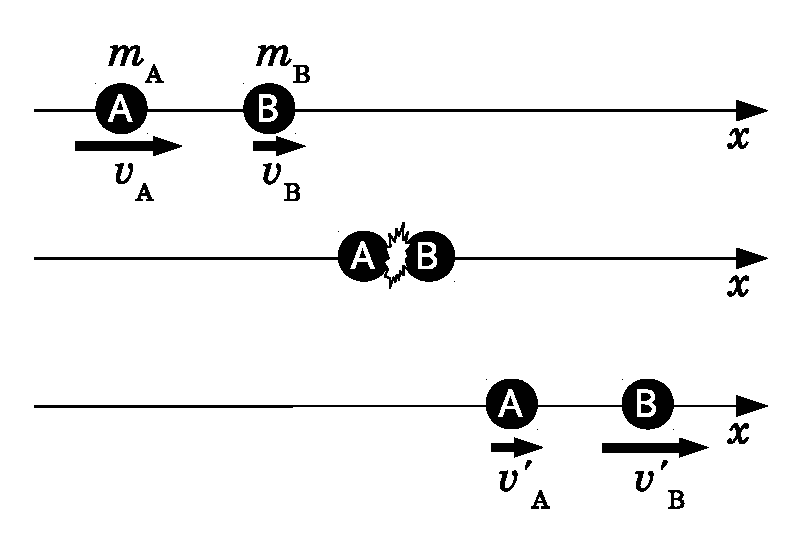
\includegraphics[width=6.5cm]{collision2.eps}
    \caption{1直線上を運動する2つの質点どうしの衝突。上: 衝突前, 中: 衝突の瞬間, 下: 衝突後}\label{fig:collision2}
\end{figure}

\begin{q}\label{q:collision2}
$x$軸上で, 2つの質点A, Bが, それぞれ速度$v_{\text{A}}$, $v_{\text{B}}$
で運動し(図\ref{fig:collision2}上), やがて互いに弾性衝突を起こし(図\ref{fig:collision2}中), 
衝突後はそれぞれ速度$v'_{\text{A}}$, $v'_{\text{B}}$で(ここではダッシュ'は微分ではなく, 
「衝突後」を表すしるし), 再び$x$軸上で運動をする
(図\ref{fig:collision2}下)。質点A, Bのそれぞれの質量を$m_{\text{A}}$, $m_{\text{B}}$とする。
2つの質点に外力は働いておらず, 2つの質点どうしに働く力(内力)は衝突時だけに働くとする。

\begin{enumerate}
\item 運動量保存則と力学的エネルギー保存則より, 以下の2つの式が成り立つことを示せ:
\begin{eqnarray}
&&m_{\text A}v_{\text A}+m_{\text B}v_{\text B}=m_{\text A}v'_{\text A}+m_{\text B}v'_{\text B}\label{eq:collision2_03}\\
&&\frac{1}{2}m_{\text A}v_{\text A}^2+\frac{1}{2}m_{\text B}v_{\text B}^2
=\frac{1}{2}m_{\text A}{v'_{\text A}}^2+\frac{1}{2}m_{\text B}{v'_{\text B}}^2\quad\quad\quad\label{eq:collision2_05}
\end{eqnarray}
\item \eref{eq:collision2_03}, \eref{eq:collision2_05}から次式を示せ:
\begin{eqnarray}
&&m_{\text A}(v'_{\text A}-v_{\text A})=-m_{\text B}(v'_{\text B}-v_{\text B})\label{eq:collision2_07}\\
&&m_{\text A}({v'_{\text A}}^2-v_{\text A}^2)=-m_{\text B}({v'_{\text B}}^2-v_{\text B}^2)\label{eq:collision2_09}
\end{eqnarray}
\item \eref{eq:collision2_09}から次式を示せ:
\begin{eqnarray}
&&m_{\text A}(v'_{\text A}-v_{\text A})(v'_{\text A}+v_{\text A})=-m_{\text B}(v'_{\text B}-v_{\text B})(v'_{\text B}+v_{\text B})\nonumber\\\label{eq:collision2_11}
\end{eqnarray}
\item \eref{eq:collision2_11}の両辺を\eref{eq:collision2_07}で割って次式を示せ:
\begin{eqnarray}
v'_{\text A}+v_{\text A}=v'_{\text B}+v_{\text B}\label{eq:collision2_13}
\end{eqnarray}
\item \eref{eq:collision2_13}を変形して次式を示せ:
\begin{eqnarray}
v'_{\text B}-v'_{\text A}=-(v_{\text B}-v_{\text A})\label{eq:collision2_14}
\end{eqnarray}
\item \eref{eq:collision2_14}を変形して次式を示せ:
\begin{eqnarray}
\frac{|v'_{\text B}-v'_{\text A}|}{|v_{\text B}-v_{\text A}|}=1\label{eq:collision2_145}
\end{eqnarray}
\end{enumerate}
\end{q}\mv\mv

\eref{eq:collision2_14}によって, ぶつかる前後で相対速度は, 向きが逆になることがわかった。
つまり, ぶつかる前には互いに近づいて来たが, ぶつかった後では互いに遠ざかっていく。これは
直感的にも明らかだ。

ぶつかった後の相対速度の大きさ$|v'_{\text B}-v'_{\text A}|$を, ぶつかる前の
相対速度の大きさ$|v_{\text B}-v_{\text A}|$で割ったものを
\underline{反発係数}\index{はんぱつけいすう@反発係数}とか跳ね返り係数と呼び, 慣習的には$e$と表す。すなわち, 
\begin{eqnarray}
e=\frac{|v'_{\text B}-v'_{\text A}|}{|v_{\text B}-v_{\text A}|}\label{eq:collision_coeff}
\end{eqnarray}
である。弾性衝突では, 
\eref{eq:collision2_145}からわかるように, $e=1$である。非弾性衝突では, 
$e$は0から1の間の値をとる。$e=0$は, 物体Bが物体Aにべちゃっとくっついてしまう場合だ。
例えばゴルフボールとゴルフクラブの衝突に関する反発係数は0.8程度である。\mv

\begin{faq}{\small\textgt{$e$って, ネイピア数(自然対数の底)じゃないんですか?}
... 記号がかぶってて, 紛らわしいけど, ここでは違います。$e$は反発係数で, 
0から1までの間の値をとります。ネイピア数は$e=2.718\cdots$だもんね。}\end{faq}\mv

\begin{q}\label{q:collision2_contin} 問\ref{q:collision2}の続きを考える。
\begin{enumerate}
\item \eref{eq:collision2_13}を使って, \eref{eq:collision2_07}から$v'_{\text B}$を消去することによって次式を示せ:
\begin{eqnarray}
v'_{\text A}=\frac{m_{\text A}-m_{\text B}}{m_{\text A}+m_{\text B}}v_{\text A}+\frac{2m_{\text B}}{m_{\text A}+m_{\text B}}v_{\text B}\label{eq:collision2_15}
\end{eqnarray}
\item \eref{eq:collision2_13}を使って, \eref{eq:collision2_07}から$v'_{\text A}$を消去することによって次式を示せ:
\begin{eqnarray}
v'_{\text B}=\frac{m_{\text B}-m_{\text A}}{m_{\text A}+m_{\text B}}v_{\text B}+\frac{2m_{\text A}}{m_{\text A}+m_{\text B}}v_{\text A}\label{eq:collision2_17}
\end{eqnarray}
\item $m_{\text A}=m_{\text B}$のとき, 次式を示せ:
\begin{eqnarray}
&&v'_{\text A}=v_{\text B}\label{eq:collision2_21}\\
&&v'_{\text B}=v_{\text A}\label{eq:collision2_23}
\end{eqnarray}
\item $m_{\text A}>>m_{\text B}$のとき, 次式を示せ:
\begin{eqnarray}
&&v'_{\text A}\fallingdotseq v_{\text A}\label{eq:collision2_25}\\
&&v'_{\text B}\fallingdotseq -v_{\text B}+2v_{\text A}\label{eq:collision2_27}
\end{eqnarray}
\end{enumerate}
\end{q}
\vspace{0.2cm}

\eref{eq:collision2_21}, \eref{eq:collision2_23}から, 
2つの質点の質量が等しければ, 弾性衝突によって速度が入れ替わる(図\ref{fig:collision24}), 
ということがわかった。追いついた方は追いつかれた方の速度になり, 追いつかれた方は
追いついた方の速度になる。
\begin{figure}[h]
    \centering
    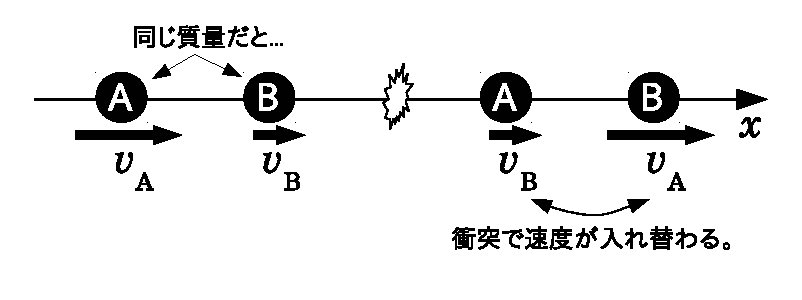
\includegraphics[width=6.5cm]{collision24.eps}
    \caption{1直線上を等速直線運動する2つの質点どうしの衝突。質量が等しく, なおかつ弾性衝突なら, 速度が入れ替わる。}\label{fig:collision24}
\end{figure}
この極端な場合は, 片方が静止してもう片方が
ぶつかってくる場合だ。ぶつかってきた方は衝突後に静止し, ぶつかられた
方がすっとんでいく。ビリヤードの経験がある人は, それを知っているだろう。\mv

ところで, \eref{eq:collision2_25}, \eref{eq:collision2_27}から, 片方の
質量が極端に大きいときは, 大きい方はほとんど速度を変えず(痛くも痒くもない), 
小さい方は激しく速度を変える(ふっとばされる), ということが
わかった(図\ref{fig:collision26})。小さな軽自動車と大きなトラックの衝突事故で, 
軽自動車に乗っていた人の方がダメージが大きいのはそのためだ。

\begin{figure}[h]
    \centering
    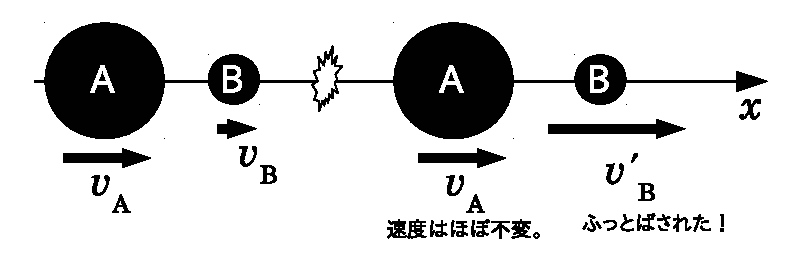
\includegraphics[width=6.5cm]{collision26.eps}
    \caption{1直線上を等速直線運動する2つの質点どうしの衝突。片方が極端に大きいときは, 小さいほうがふっとばされる。}\label{fig:collision26}
\end{figure}

%
\begin{q}\label{q:ball_bound}
ボールを高さ$h_0$から初速度0で真下に落として, バウンドさせる。
ボールと地面の間の反発係数を$e$としよう。空気抵抗やボールの回転は無視する。
\begin{enumerate}
\item ボールが地面につく直前の速度を$v_0$とする。力学的エネルギー保存則から次式を示せ:
\begin{eqnarray}v_0^2=2gh_0\label{eq:ball_bound1}\end{eqnarray}
\item ボールが地面で跳ね返った直後の速度を$v_1$とする。次式を示せ:
\begin{eqnarray}|v_1|=e|v_0|\label{eq:ball_bound2}\end{eqnarray}
\item ボールは地面で跳ね返ったあと上向きに運動し, いずれある点(それを到達点と呼ぼう)
に達してまた落ち始める。そのときの到達点の高さを$h_1$として, 次式を示せ:
\begin{eqnarray}v_1^2=2gh_1\label{eq:ball_bound3}\end{eqnarray}
\item 次式を示せ:
\begin{eqnarray}h_1=e^2h_0\label{eq:ball_bound4}\end{eqnarray}
\item そのまま放っておけば, またボールは地面に衝突して跳ね返り, また落ちて地面に衝突して
跳ね返り, ...ということを繰り返すだろう。$n$を1以上の整数として, ボールが$n$回バウンド
したあとの到達点の高さを$h_n$とすると, 次式を示せ:
\begin{eqnarray}h_n=e^{2n}h_0\label{eq:ball_bound5}\end{eqnarray}
\item $e=0.8$, $h_0=10$~mのとき, 到達点の高さが0.1~m以下になるまでに, 何回バウンドするか? 
\end{enumerate}
\end{q}
\mv

\begin{q}\label{q:balls_bound}
2つのボールを, わずかに隙間をあけて縦に重ねて, 高さ$h$から(初速度0で)
真下の地面に落とし, バウンドさせる。下のボールを「ボールA」とし, 
その質量を$m_{\text A}$とする。上のボールを「ボールB」とし, 質量を$m_{\text B}$とする。
ボールBはボールAよりはるかに小さく, $m_{\text A}>>m_{\text B}$とする。ボールAと
地面の衝突や, ボールAとボールBの衝突は弾性衝突であるとする。
重力加速度を$g$とする。上向きに座標軸をとる。

\begin{figure}[h]
    \centering
    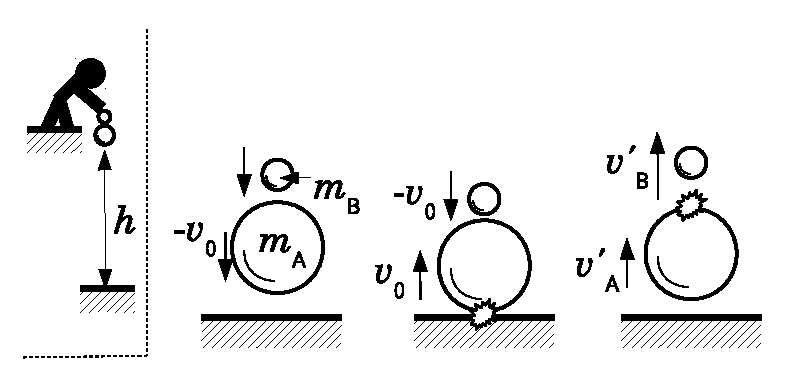
\includegraphics[width=7cm]{balls_bound.eps}
    \caption{2段のボールの落下と跳ね返り。問\ref{q:balls_bound}。}\label{fig:balls_bound}
\end{figure}

\begin{enumerate}
\item 地面に衝突する直前(図\ref{fig:balls_bound}中左)のボールAの速度の大きさを$v_0$とする。$v_0=\sqrt{2gh}$であることを示せ。
\item ボールAが地面に衝突して跳ね返った直後は, ボールBはまだボールAの上空にあるとする(図\ref{fig:balls_bound}中右)。このときのボールAの
速度を$v_{\text A}$, ボールBの速度を$v_{\text B}$とする。次式を示せ:
\begin{eqnarray}
&&v_{\text A}=v_0\\
&&v_{\text B}=-v_0
\end{eqnarray}
\item その直後に, ボールBはボールAに衝突して跳ね返る(図\ref{fig:balls_bound}右端)。衝突直後のボールBの速度を$v'_{\text B}$とする。
これらの一連の衝突は, 地面付近の狭い範囲で起きるので, 重力によるポテンシャルエネルギーの変化を
無視しよう。すると\eref{eq:collision2_27}が成り立つことから, 次式を示せ:
\begin{eqnarray}
v'_{\text B}\fallingdotseq 3v_0\label{eq:balls_bound4}
\end{eqnarray}
\item ボールBは, ボールAに衝突して跳ね返ったあと, もとの落下開始点(高さ$h$)の何倍の高さまで飛び上がるか?
\end{enumerate}
\end{q}
\mv

\section{回転運動再考}

ところで, 太陽のまわりを地球が円運動(公転)している系を考えよう。太陽と地球だけの系
には外力は働かないので, 運動量保存則から, 全運動量は一定のはずだ。さて, 地球の速度は, 
大きさこそ一定であっても, 円軌道に沿って時々刻々と向きを変える。すると, 地球の運動量は, 
大きさこそ一定であっても, 時々刻々と向きが変わるはずだ。一方, 太陽は静止しているから
運動量は無い。ということは, 全運動量は地球の運動量だけだ。ということは, 全運動量
が時々刻々と変化している, ということになる!! これは運動量保存則に矛盾している。どこが
間違っているだろうか?

実は, この考察は, 「太陽は静止しているから運動量は無い」から後が間違っている。
地球が太陽から引力を受けるように, 太陽も地球から引力を受ける(「作用・反作用の法則」)。
その力によって, 太陽も, 小さいながらも円運動するのだ。しかもその運動量は, 絶えず地球の運動量とは逆向きで
大きさが同じであるため, 太陽と地球の全運動量は0で一定なのである\footnote{ただし
太陽と地球の重心に対して静止している座標系で見た場合。}。
\hv



\begin{exq}\label{q:balls_bound_n} さっきは
ボールを2段にして落としたが, こんどはボールをもっとたくさん用意して重ねて
落としてみよう。$n$個のボールを縦に重ねて, 前問と同じように高さ$h$から
落とす。ボールは上のものほど軽く, 隣りあう上下のボールは, 上のボールのほうが
下のボールよりはるかに小さい(軽い)とする。最下部のボールが地面に弾性衝突して跳ね返ったあと, 
ボール同士は多段階に弾性衝突する(図\ref{fig:balls_bound_n})。最後に最上部のボールが跳ね上がるときのその
ボールの速度を$v'_n$とする。

\begin{figure}[h]
    \centering
    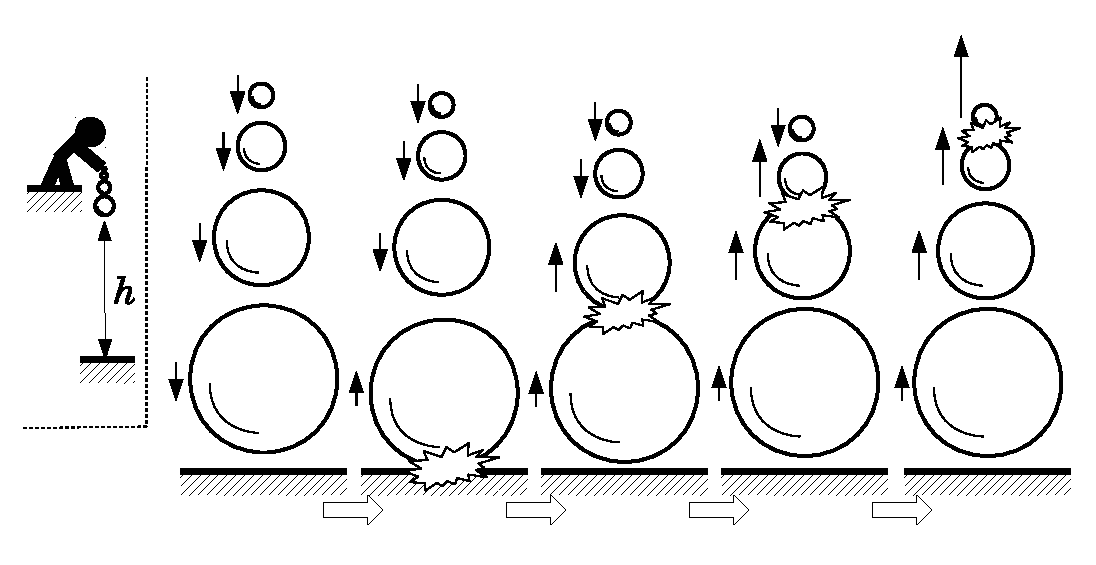
\includegraphics[width=7cm]{balls_bound_n.eps}
    \caption{多段のボールの落下と跳ね返り。問\ref{q:balls_bound_n}。}\label{fig:balls_bound_n}
\end{figure}

\begin{enumerate}
\item 次式を示せ:
\begin{eqnarray}
v'_n\fallingdotseq (2^n-1)v_0\label{eq:balls_bound_n3}
\end{eqnarray}
\item 最上部のボールは, もとの落下開始点(高さ$h$)の何倍の高さまで飛び上がるか?
\item ボール群を$h=5$~mから落下させ, 最上部のボールを宇宙の彼方まで
飛ばすには, ボールを10段程度にすればよいことを示せ。(ヒント: 第2宇宙速度)
\end{enumerate}
\end{exq}

\begin{exq} テニスのトップ選手の打つボールの速さは200~km/h程度である。
フェデラー選手が200~km/hのサービスを打ち, それを錦織圭選手が200~km/hで打ち返した。
その際, 錦織選手のラケットとボールが接触している時間は3.0~msだった。その間、
ボールに働いた力の大きさを見積もれ。また, そのような大きな力が発生するにもかかわらず, 
錦織選手の右腕が壊れないのはなぜだろう? ただしテニスボールの質量を60~gとする。\end{exq}

\begin{exq} 宇宙空間で直線上を加速しながら進むロケットの運動を考えよう。
ロケットにはたくさんの燃料が積まれている。燃料込みでのロケットの質量を$M$とする。
ロケットは, 相対速度$u$で, 燃料を後方に噴射することによって加速して
いく。と同時に, 噴射した燃料のぶんだけ質量$M$は減る。すなわち, ロケットは
質量が減るほど, 速度が増す。ロケットの初期速度を0, 初期の質量を$M_0$とする。
ロケットの速度$v$と質量$M$の関係を求めよ。ヒント: ある瞬間と, そこから少し経った
瞬間での, 運動量保存則を考える。ロケットの質量$M$は, $M+dM$に変わる($dM<0$)。
$dM$は出て行った微小な燃料の質量(にマイナスをつけたもの)。燃料は, $v-u$という速度で
ロケットから離れる。\end{exq}


\section{解答}
% $m_{\text A}=m_{\text B}=1$kgとし, 時刻$t_0$で$A$は$x$軸方向に1m/s, $B$は$y$軸方向に
\noindent{\textbf{答}}\ref{q:collision0}
\begin{enumerate}
\item $m_{\text A}=m_{\text B}=1$~kg, 
${\bf v}_{\text A}=(1\text{ m s}^{-1}, 0\text{ m s}^{-1})$, \\
${\bf v}_{\text B}=(0\text{ m s}^{-1}, 1\text{ m s}^{-1})$
として\eref{eq:2body_adhere}に代入すると, 
${\bf v}=(0.5\text{ m s}^{-1}, 0.5\text{ m s}^{-1})$。
\item $|{\bf v}|=|(0.5\text{ m s}^{-1}, 0.5\text{ m s}^{-1})|=0.71\text{ m s}^{-1}$。
\end{enumerate}

\noindent{\textbf{答}}\ref{q:def_rikiseki} 略。
\mv

% 3つの質点$A, B, C$が互いに内力のみを受けて運動する系でも, 全運動量が保存する
\noindent{\textbf{答}}\ref{q:3body_momentum}
(略証)
\begin{eqnarray*}
m_{\text A}{\bf v}_{\text A}(t_1)-m_{\text A}{\bf v}_{\text A}(t_0)=\int_{t_0}^{t_1}({\bf F}_{\text {AB}}+{\bf F}_{\text {AC}})dt\\
m_{\text B}{\bf v}_{\text B}(t_1)-m_{\text B}{\bf v}_{\text B}(t_0)=\int_{t_0}^{t_1}({\bf F}_{\text {BA}}+{\bf F}_{\text {BC}})dt\\
m_{\text C}{\bf v}_{\text C}(t_1)-m_{\text C}{\bf v}_{\text C}(t_0)=\int_{t_0}^{t_1}({\bf F}_{\text {CA}}+{\bf F}_{\text {CB}})dt
\end{eqnarray*}
これらの式を辺々加える。作用反作用の法則から${\bf F}_{\text {AB}}+{\bf F}_{\text {BA}}$
などは${\bf 0}$になるので, 結局, 
\begin{eqnarray*}
&&m_{\text A}{\bf v}_{\text A}(t_1)+m_{\text B}{\bf v}_{\text B}(t_1)+m_{\text C}{\bf v}_{\text C}(t_1)\\
&&=m_{\text A}{\bf v}_{\text A}(t_0)+m_{\text B}{\bf v}_{\text B}(t_0)+m_{\text C}{\bf v}_{\text C}(t_0)
\end{eqnarray*}

% 
\noindent{\textbf{答}}\ref{q:collision1}
\begin{enumerate}
\item $A, B$ともに同じ運動エネルギー: 0.5 Jをもつ。従って全運動エネルギーは, 1 J。
\item $(m_{\text A}+m_{\text B})|{\bf v}|^2/2=0.5$ J。
\end{enumerate}

% 弾性衝突とは何か? 
\noindent{\textbf{答}}\ref{q:elastic_collision}
衝突によって運動エネルギーが失われない衝突。

% $x$軸上に質量$m_{\text A}$の質点$A$が静止している。ここに, $x$軸の負のほうから, 
\noindent{\textbf{答}}\ref{q:collision2} 略。

\noindent{\textbf{答}}\ref{q:collision2_contin}
(1), (2), (3)は略(実直に計算すれば導出できる)。\mv
(4) \eref{eq:collision2_15}, \eref{eq:collision2_17}の分子分母を$m_{\text A}$で割ると, 
\begin{eqnarray*}
&&v'_{\text A}=\frac{1-m_{\text B}/m_{\text A}}{1+m_{\text B}/m_{\text A}}v_{\text A}+\frac{2m_{\text B}/m_{\text A}}{1+m_{\text B}/m_{\text A}}v_{\text B}\\
&&v'_{\text B}=\frac{m_{\text B}/m_{\text A}-1}{1+m_{\text B}/m_{\text A}}v_{\text B}+\frac{2}{1+m_{\text B}/m_{\text A}}v_{\text A}
\end{eqnarray*}
となる。ここで, $m_{\text A}>>m_{\text B}$なので, $m_{\text B}/m_{\text A}\fallingdotseq0$とすると, 上の2つの式は, 
\begin{eqnarray*}
&&v'_{\text A}\fallingdotseq \frac{1-0}{1+0}v_{\text A}+\frac{2\times0}{1+0}v_{\text B}=v_{\text A}\\
&&v'_{\text B}\fallingdotseq \frac{0-1}{1+0}v_{\text B}+\frac{2}{1+0}v_{\text A}=-v_{\text B}+2v_{\text A}
\end{eqnarray*}
となり, 与式を得る。
\vspace{0.2cm}


% ボールを高さ$h_1$から(初速度0で)真下に地面に落として, バウンドさせる。
\noindent{\textbf{答}}\ref{q:ball_bound}
\begin{enumerate}
\item 地面を基準点とする。ボールを手放した瞬間は, 重力によるボールのポテンシャルエネルギーは$mgh_0$で, 運動エネルギーは初速度0なので$0$。
従って力学的エネルギーは$mgh_0$。一方, 地面につく直前は, ボールのポテンシャルエネルギーは$0$で, 運動エネルギー
は$mv_0^2/2$。従って力学的エネルギーは$mv_0^2/2$。力学的エネルギー保存則より, $mgh_0=mv_0^2/2$。ここから与式を得る。
\item 略。($e$の定義から)
\item 略。(\eref{eq:ball_bound1}と同様)
\item 略。(\eref{eq:ball_bound1}, \eref{eq:ball_bound2}, \eref{eq:ball_bound3}より$v_0, v_1$を消去)
\item 前小問と同様に, $h_n=e^2h_{n-1}$。これは公比$e^2$の等比数列。従って与式を得る。(数学リメディアル教材参照)
\item $h_0=10$~mで, $h_n=e^{2n}h_0<0.1$~mより, \\
$e^{2n}<0.01$
となる。$e=0.8$だから, $0.8^{2n}<0.01$。$n=10$のとき
$0.8^{2n}=0.0115>0.01$。$n=11$のとき$0.8^{2n}=0.0074<0.01$。従って, $n=11$, つまり11回バウンドする。
\end{enumerate}
\vspace{0.2cm}


%
\noindent{\textbf{答}}\ref{q:balls_bound}
(1) ボールAについて, 落下から地面での衝突の直前までを考えると, 力学的エネルギー保存則より, 
\begin{eqnarray}
\frac{1}{2}m_{\text{A}}v_0^2=m_{\text{A}}gh\label{eq:balls_bound_ans2}
\end{eqnarray}
これを$v_0$について解けば与式を得る。\mv
(2), (3)は略(誘導に従って実直に計算すれば導出できる)。\mv
(4) ボールBについて, (1)と同様に考えれば, 次式のようになる: 
\begin{eqnarray}
\frac{1}{2}m_{\text{B}}v_0^2=m_{\text{B}}gh\label{eq:balls_bound_ans3}
\end{eqnarray}
一方, 最高到達点の高さを$H$とし, 衝突直後から最高点到達までを考えると, 力学的エネルギー保存則より, 
\begin{eqnarray*}
\frac{1}{2}m_{\text{B}}{v'_{\text B}}^2=m_{\text{B}}gH
\end{eqnarray*}
ここで(3)より, $v'_{\text B}=3v_0$だから, 
\begin{eqnarray}
\frac{9}{2}m_{\text{B}}v_0^2=m_{\text{B}}gH\label{eq:balls_bound_ans4}
\end{eqnarray}
となる。\eref{eq:balls_bound_ans4}の辺々を\eref{eq:balls_bound_ans3}の辺々で割ると, 
$9=H/h$となる。すなわち, $H=9h$。すなわち, もとの高さの9倍まで上がる。
\mv


\section{補遺: 量子のエネルギー}

実は, 我々が学んでいる力学(ニュートン力学)は, 分子や原子などの小ささになると, 
効力を失う。そのようなスケールを支配するのは, 「量子力学」という, 全く別な
理論だ。量子力学は物理現象や物理的存在の捉え方がニュートン力学とは
まるきり違っている。ニュートン力学では, 「速度」とか「力」とか
が大事な概念だったが, 量子力学では, それらにあまりこだわらない。というか, 
量子力学のスケールでは, そういうことにこだわっても仕方ないようなふうに
物体や現象が存在し, 振る舞うのである\footnote{量子力学では, 
速度のかわりに運動量, 力のかわりにポテンシャルエネルギーが, 
それぞれ重要な役割を担う。}。

それがどういうことなのかを理解するには, どうしても高度な数学が必要だ。
ある著名な物理学者は「神は非常に高度な数学者であり, 宇宙を作る時に
極めて高級な数学を使ったのだ」と言ったほどだ。我々は神様ほど高度な数学者では
ないのでどうしようもないが, それでも「化学II」「化学結合論」などの授業で
量子力学が出てくる。そこで, 量子力学のほんの入り口をここで学ぼう。
以下の話では, 「なぜそうなるのか」を説明することはできない。
自然はともかくそのように振る舞うのだ。

まず, 量子力学では, 物体や現象を「量子」という概念で把握する。電子や原子や
光は, いずれも「量子」として振る舞う。量子は, 1個2個と数えられるような
離散的な存在であり, その存在のあり方は, 「状態ベクトル」という数学的な
概念で表現される。その「ベクトル」という言葉から, 平面ベクトルや空間ベクトル
のようなもの, つまり「大きさと向きを持つもの」(矢印)を君は想像するかもしれないが, 
そうではない。状態ベクトルは, そういうベクトルとは違う, もっと抽象的な概念だ。
その「状態ベクトル」を, 位置$(x, y, z)$の関数として
表現したものを「波動関数」と言う\footnote{「ベクトル」が「関数」になる? どういうこと?
 と君は思うかもしれないが, 「関数もベクトルの一種だ」という話をどこかで
小耳に挟まなかっただろうか。}。波動関数は, 「シュレーディンガー方程式」
という小難しい微分方程式に従うことがわかっている。

量子が, ある特定のエネルギーを持つ状態にあるとき, 
シュレーディンガー方程式は「行列の固有値と固有ベクトル
を求める問題」(数学リメディアル教材でやった!)に帰着できる。
その「固有値」がエネルギーに該当し, 「固有ベクトル」が
状態ベクトル(それを位置で表現するならば波動関数と言っても
良い)に対応する(なのでそのような状態やそのエネルギーを
「固有状態」「固有エネルギー」と呼ぶ)。このとき, 状態ベクトル
は時刻$t$に対して振動的に依存する。その振動の角速度を
$\omega$とすると, 量子のエネルギー$E$は(それは行列の固有値
でもあるのだが), 
\begin{eqnarray}
E=\frac{h}{2\pi}\omega\label{eq:E_h_omega}
\end{eqnarray}
となる。ここで$h$は「プランク定数」と呼ばれる定数で, 
\begin{eqnarray}
h=6.626068\times10^{-34}\text{ J s}
\end{eqnarray}
である。$h/(2\pi)$は量子力学で頻繁にあらわれるので, $2\pi$をいちいち
書くのがめんどくさくなって, 物理学者達は, それを$\hbar$と
書き表すことにした(これを「エイチバー」と読む)。すなわち, 
\begin{eqnarray}
\hbar:=\frac{h}{2\pi}\quad\quad\text{(定義)}\label{eq:def_hbar}
\end{eqnarray}
である。すると, \eref{eq:E_h_omega}は次式のように書ける:
\begin{eqnarray}
E=\hbar \omega\label{eq:E_hbar_omega}
\end{eqnarray}

さて, 数学的な理由から, 波動関数は, 空間の中を振動しながら
広がっていくような性質を持つ。だから, 量子は「粒子の性質と
波の性質の両方を持つ」と言われることが多い。

特に, 光はそもそも電場と磁場の振動が空間を伝わる波なので, そのような
「波」のイメージが強い。実際, 光の状態ベクトル(波動関数)の振動の
角速度$\omega$は, 電場や磁場の振動の角速度$\omega$そのものである。
光速を$c$とすると, 波としての光は, 周期$2\pi/\omega$の間に速さ$c$で
波長$\lambda$だけ進むので, 
\begin{eqnarray}
\frac{2\pi}{\omega}\,c=\lambda
\end{eqnarray}
という式が成り立つ。この式を使って\eref{eq:E_h_omega}の$\omega$を消去
すると, 光の量子(それを光量子とか光子という)のエネルギーは, 
\begin{eqnarray}
E=\frac{hc}{\lambda}\label{eq:E_photon}
\end{eqnarray}
となる。この式はよく教科書に出てくるが, 注意すべきなのは, 
\underline{この\eref{eq:E_photon}は光子にしか成り立たない}, 
ということだ。光子以外にも, 様々な量子が世の中には存在し(電子とか), それぞれが波動関数の
角速度とか波長という特徴を持つのだが, \eref{eq:E_photon}は
必ずしも成り立たなくても, \eref{eq:E_h_omega}や\eref{eq:E_hbar_omega}
は光子も含めていかなる量子にも成り立つ。\mv
